\section{Weighting data and calculating indices}
\label{sec:weighting_and_calculating}

\begin{figure}
    \centering
    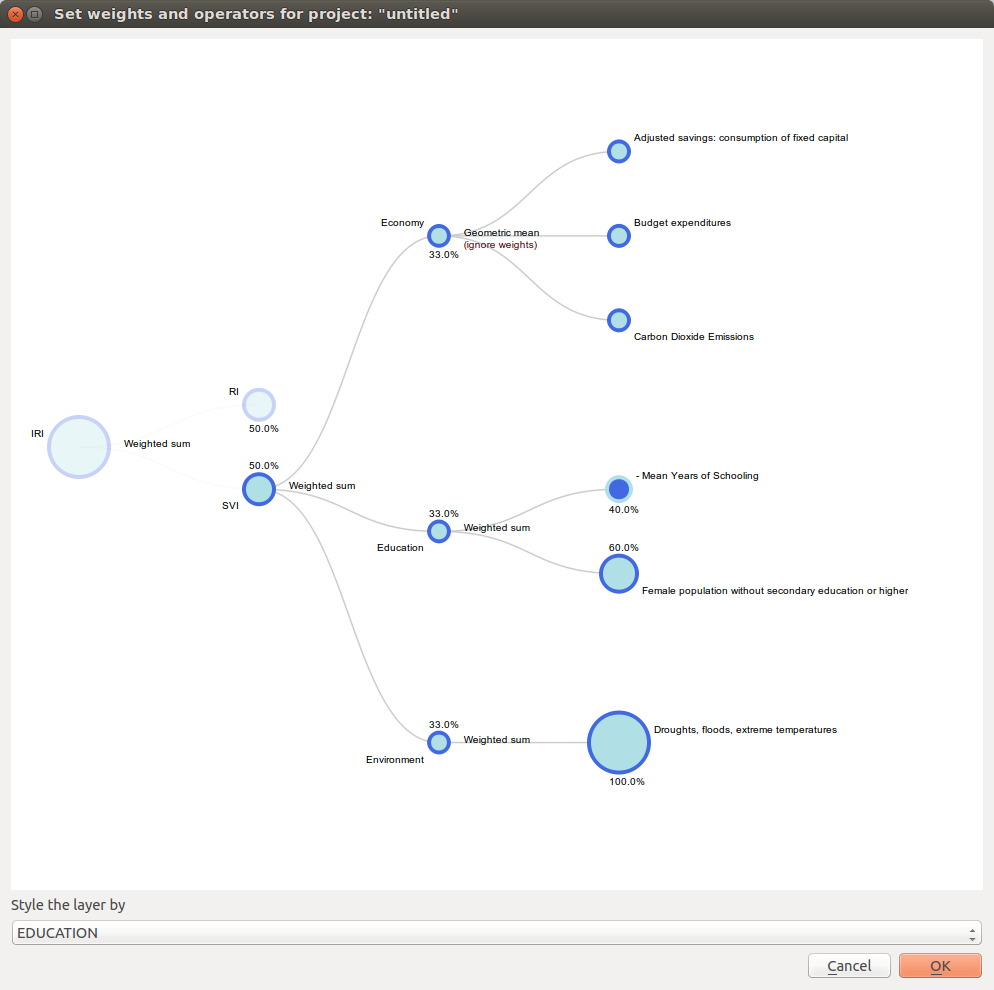
\includegraphics[width=\textwidth]{../images/image06}
    \caption{Tree chart structure for the development of composite indicators}
    \label{fig:weighting_and_calculating}
\end{figure}

Central to the construction of composite indicators is the need to meaningfully
combine different data dimensions, and consideration must be given to weighting
and aggregation procedures. Most composite indicators rely on equal weighting
largely for simplicity. Equal weighting, however, implies that all variables
within the composite indicator are of equal importance when this may not
actually be the case. The issue of aggregation is similar to the weighting
process. Different aggregation rules may be applied depending on the underlying
theoretical framework chosen by the user for the modelling process.
Sub-indicators may be summed up (linear aggregation) for instance, multiplied,
or geometrically aggregated to correct for compensability (i.e.\ the possibility
of offsetting a deficit in some dimension with an outstanding performance in
another). Each technique has specific consequences, implies different
assumptions, and could ignore or incorporate weights.

The `Weight data and calculate indices' application
(Figure~\ref{fig:weighting_and_calculating}) is the key module of the IMRT\@. It
contains the model building functionality of the IRMT, and it is used to
create, edit, and manage composite indicator(s) and integrated risk model
development. The `Weight data and calculate indices' application provides users
with an intuitive way to develop composite models by building and editing the
selected project definition through the use of a dynamic graphical interface
that was developed explicitly to guide the construction of composite indicators
in a manner that is simple, visual, and straight-forward. The latter is
accomplished through a window that embeds a web browser in which a javascript
D3 tree chart is rendered (see Figure~\ref{fig:weighting_and_calculating}).
This tree chart structure (or weighting and aggregation tree) defines a
workflow that strings together sequences of steps to describe how variables are
combined together to obtain the composite indices.  

\begin{figure}
    \centering
    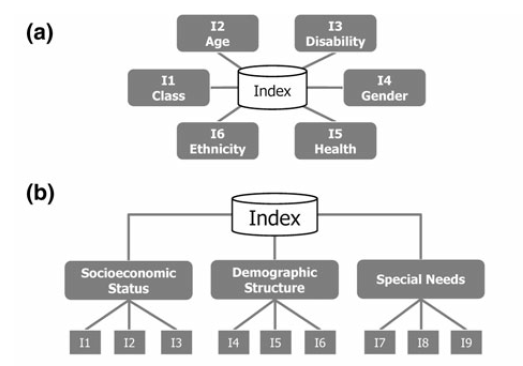
\includegraphics[width=\textwidth]{../images/image19}
    \caption{Composite indicator types (adapted from: Tate, E.C. 2012.
    Social vulnerability indices: a comparative assessment using uncertainty
    and sensitivity analysis, Natural Hazards, 63(2): 325-347)}
    \label{fig:composite_indicator_types}
\end{figure}

Currently, the IRMT supports the development of two composite model types: a)
deductive and, b) hierarchical (Figure~\ref{fig:composite_indicator_types}).
Deductive models typically contain fewer than ten indicators that are
normalized and aggregated to create an index. Hierarchical models typically
employ ten to twenty indicators that are separated into groups (sub-indices)
that share the same underlying dimension of a concept (in this case
socio-economic parameters of earthquake risk such as population, economy,
infrastructure, education, and governance).  Individual indicators are
aggregated into sub-indices (e.g.\ population, economy, etc), and the
sub-indices are aggregated to form a final composite index (e.g.\ a social
vulnerability or integrated risk index). The tree structure of the `Weight data
and calculate indices' application encourages the development of hierarchical
models of integrated risk. The starting point is a `root node' that corresponds
to the development of a hierarchical model that can be: 1) an `Integrated Risk
Index' (IRI) which is a function of the aggregation of a `Social Vulnerability
Index' (SVI) and a `Risk Index' (RI); or 2) a `Social Vulnerability Index'
(SVI) that is the result of the aggregation of various sub-indicators defined
by the user (e.g.\ Economy, Education, and Environment as shown within
Figure~\ref{fig:weighting_and_calculating}).  The tree can be modified
dynamically by adding or removing nodes, `inverting' variables, setting a
weight to each variable or node and choosing the operators to be used to
combine variables together.

Whenever `Update' or `Update and close' are clicked, the project definition is
updated and the composite indices are re-calculated. As a consequence, the map
is rendered and styled accordingly. This allows the user to have an immediate
feedback on how the map changes depending on how the project definition is set.
Such automatic re-calculations and rendering can take some time, depending on
the complexity of the project and number of enumerations units analysed.

The main functional elements of the weighting and aggregation tree are
discussed in the subsections below.


\subsection{Adding a node}

Individual nodes correspond to aggregated composite indicators within the
weighting and aggregation tree. To add a node (i.e.\ a composite sub-indicator)
within the tree, it is possible to begin by left-clicking on the default node
(i.e.\ SVI).  Clicking on the default SVI node allows the addition of multiple
new sub-indicators, each with its own user-provided name (note that it is not
possible to add nodes stemming from the IRI). When a newly created node is
clicked, a new dialog is initiated to give users the option to select the
variables available in the layer (and not already used in the node) to populate
the sub-indicator being under construction. Please note that the SVI can be
calculated if each socioeconomic sub-indicator has at least one variable. In
order to add an indicator to one of the socioeconomic sub-indicators, you can
click on the corresponding node. When adding an indicator to the RI, or to one
of the socioeconomic sub-indicators, the description of the node will be
automatically set to be equal to the name of the corresponding layer's
variable. Users can edit this description, however, by clicking on the text
displayed next to the node in the tree and then by clicking within the
corresponding textbox to change the text.


\subsection{Removing a node}

In order to remove one of the nodes from the tree, users can perform a
right-click on that node. A popup dialog window will ask you to confirm if you
really intend to delete the node and all of its `children' (the lower level
nodes connected to it). Please note that removing a node from the tree will not
delete the corresponding field from the layer.


\subsection{Setting the operators to be used to combine nodes together
(variable aggregation)}
\label{sec:setting_operators}

On the right of each node, the tree indicates the name of the operator to be
used to combine (or aggregate) the `children' of such node. By clicking on the
operator's name, a dialog to set weights and operators is opened. The same
happens when clicking on the name of one of the children nodes. The operator
can be chosen from a dropdown menu. Some operators (e.g., `Weighted sum') take
into account the weights applied to the child nodes. Other operators (e.g.,
`Average (ignore weights)') do not take into account weights. When the chosen
operator is one of the latter, the child nodes will be rendered on the
graphical display all with the same radius and their weights will not be
rendered (see Figure~\ref{fig:weighting_and_calculating} for a demonstration of
how the radius of nodes corresponds with the respective weights of variables).
Otherwise, the radius of a node is proportional to its weight, and the weight
is rendered next to the node.


\subsection{Setting weights}

Central to the construction of composite indicators in the need to combine data
into meaningful dimensions which implies decisions on weighting. The dialog to
set weights is opened in the same way as described in
Section~\ref{sec:setting_operators}. Several weighting techniques are
available, and some make use of statistical models.  For the IRMT we
implemented a simple solution to weighting that is often based on the results
of participatory approaches. A weight can be edited manually by clicking on its
value and overwriting it with a new value. A weight can also be edited by
clicking on the spinner's arrows to increase or decrease the weight.  By
clicking `Update', the weights will be re-calculated in order to make them sum
to 1. In other words, if you have 3 variables and you set their weights to 1, 2
and 5 and you press `Update', the weights will be re-calculated to be
respectively 0.125, 0.250 and 0.625, keeping the same proportion between each
other, and summing to 1.


\subsection{Inverting a variable}

The dialog to invert variables is opened in the same way as described in
Section~\ref{sec:setting_operators}. If a variable contributes in a `negative'
way to the composite indicator (e.g., a higher education corresponding to a
lower social vulnerability), it is possible to indicate such an inverse
relationship by pressing the `Invert' button next to the variable name. The
effect on a composite indicator in response to this decision process and
setting is that each value of the `inverted' variables will be to multiplied by
-1 each time the variables themselves are used in a calculation.  Please note
that the layer's field will keep holding the original value of the variable,
and that the inversion will be performed on-the-fly for the purpose of the
calculation.


\subsection{Assigning a new name to a variable}

The dialog to assign a new name to a variable is also opened in the same way as
described in Section~\ref{sec:setting_operators}. By clicking on the variable's
name, a popup dialog asks users to insert the new name. The project definition
will be updated accordingly, linking the layer's fieldname with the modified
description.


\subsection{Styling the layer by a chosen field}

The dropdown menu on the bottom of the `Set weights and operators' module can
be used to choose fields within a layer, i.e., fields other than those
delineated within the project definition to be symbolized, allowing all fields
in a layer to be to be symbolized on-the-fly.  This can be useful, for
instance, to map the values calculated for different sub-indicators, or even
individual variables if they are of interest. By default, the selection is
blank. In the default case, the tool will adopt the following convention: 1) if
the IRI can be computed, then the layer will be symbolized according to it; 2)
otherwise, if the SVI can be computed, then it will be used as the default case
for symbolization in the absence of IRI; 3) otherwise, the convention will
apply with respect to the RI; and 4) if none of main sub-indicators can be
calculated, then the layer will not be re-styled unless the user uses the
dropdown menu to specify a specific symbolization field.
